

\begin{center}
\begin{tikzpicture}
%\draw[fill=gray!23,gray!23](0,0) rectangle (7,5);
%\draw[step=0.5cm,gray,very thin] (0,0) grid (12,5); %background grid

\node[] at (0.1,2.7) {$\tau$};
\draw[line width=1mm] (0.5,1.5) -- (0.5,3.5) ;   
\draw [->] (0,2.5) -- (0.45,2.5);
\draw [->] (0,2) -- (0.45,2);
\draw [->] (0,3) -- (0.45,3);

\draw[thick] (0.5,2.5) -- (2,2.5) ;   
\draw[thick] (2.5,2.5) -- (5,2.5) ;   
\draw[thick] (5.5,2.5) -- (7.5,2.5) ;   
\draw[thick] (10.5,2.5) -- (12,2.5) ;   

% v damper
\draw[thick] (1.5,3) -- (2.5,3) -- (2.5,2) -- (1.5,2);  
% ds damper
\draw[thick] (4.5,3) -- (5.5,3) -- (5.5,2) -- (4.5,2);  
% m damper
\draw[thick] (8.5,4) -- (9.5,4) -- (9.5,3) -- (8.5,3);  

\node[] at (2,1.6) {$\eta_{\color{orange}v}$};
\node[] at (5,1.6) {$\eta_{\color{green}ds}$};
\node[] at (9,4.4) {$\eta_m$};

\draw[thick] (9,3.5) -- (7.5,3.5) -- (7.5,1.5) -- (8,1.5);  
\draw[thick] (9.5,3.5) -- (10.5,3.5) -- (10.5,1.5) -- (10,1.5);  

\draw[thick] (8,1.5) -- (8.5,1.4) -- (9.5,1.4) ;   
\draw[thick] (8.5,1.6) -- (9.5,1.6) -- (10,1.5) ;   

\node[] at (9,1.92) {$Y$};

%wall
\draw[line width=2mm] (12,1.5) -- (12,3.5) ;   
\draw[thick] (12,1.5) -- (12.25,1.75) ;   
\draw[thick] (12,1.75) -- (12.25,2) ;   
\draw[thick] (12,2) -- (12.25,2.25) ;   
\draw[thick] (12,2.25) -- (12.25,2.5) ;   
\draw[thick] (12,2.5) -- (12.25,2.75) ;   
\draw[thick] (12,2.75) -- (12.25,3) ;   
\draw[thick] (12,3) -- (12.25,3.25) ;   
\draw[thick] (12,3.25) -- (12.25,3.5) ;   

\draw[>=triangle 45, <->] (0.5,0.95) -- (3.5,0.95);
\draw[>=triangle 45, <->] (3.5,.95) -- (6.5,0.95);
\draw[>=triangle 45, <->] (6.5,0.95) -- (12,0.95);
\node[] at (2,0.75)   {$\dot\varepsilon_{\color{orange}v}$};
\node[] at (5,0.75)   {$\dot\varepsilon_{\color{green}ds}$};
\node[] at (9.5,0.75) {$\dot\varepsilon_{\color{blue}vp}$};

\end{tikzpicture}

\end{center}
This rheology would be called visco-viscoplastic.
The algorithm goes then as follows:
\begin{enumerate}
\item Assume we know $\eta_v$ and $\dot\varepsilon_T$ (from previous iteration), as well as the plasticity parameters $Y$ and $\eta_m$.
\item if $2 \eta_v \dot\varepsilon_T < Y$ the stress is below the yield stress value and plasticity is not active. Use $\eta_v$ in the material model and $\dot\varepsilon_v=\dot\varepsilon_T$.

\item if $2 \eta_v \dot\varepsilon_T > Y$ the stress is above the yield value, which is not allowed. In this case the plastic element is 'switched on'. In that case the viscous damper is in series with the (visco)plastic element. The former deforms with a strain rate $\dot\epsilon_v$ while the latter with $\dot\epsilon_{vp}$ (both under the same stress $\tau$) and we have  $\dot\varepsilon_T = \dot\varepsilon_v  + \dot\varepsilon_{vp}$. 

\begin{eqnarray}
\dot\varepsilon_T 
&=& \dot\varepsilon_v + \dot\varepsilon_{vp}  \nonumber\\
&=& \dot\varepsilon_v + \frac{\tau}{2 \eta_{vp}} \nonumber\\
&=& \dot\varepsilon_v + \frac{\tau}{2 \left( \frac{Y}{2\dot\varepsilon_{vp}} + \eta_m  \right)} \nonumber\\
&=& \dot\varepsilon_v + \frac{\tau}{2 \left( \frac{Y}{2(\dot\varepsilon_T-\dot\varepsilon_v)}+\eta_m\right)} \nonumber\\
\dot\varepsilon_T - \dot\varepsilon_v 
&=& \frac{\tau}{2 \left( \frac{Y}{2(\dot\varepsilon_T-\dot\varepsilon_v)}+\eta_m\right)} \nonumber\\
2 (\dot\varepsilon_T - \dot\varepsilon_v)
\left( \frac{Y}{2(\dot\varepsilon_T-\dot\varepsilon_v)}+\eta_m\right) &=& \tau \nonumber\\
Y +  2(\dot\varepsilon_T - \dot\varepsilon_v) \eta_m &=& \tau \nonumber\\
Y +  2(\dot\varepsilon_T - \frac{\tau}{2 \eta_v}) \eta_m &=& \tau \nonumber\\
Y +  (2\eta_v \dot\varepsilon_T - \tau) \frac{\eta_m}{\eta_v} &=& \tau \nonumber\\
Y +  2\eta_m \dot\varepsilon_T  &=& \tau (1 + \frac{\eta_m}{\eta_v} ) \nonumber
\end{eqnarray}
and finally 
\begin{equation}
\tau  = \frac{Y + 2 \eta_m \dot\varepsilon_T} {1+ \frac{\eta_m}{\eta_v} }
\end{equation}
Note that this solution exists even when $\eta_m=0$, and then rather logically $\tau=Y$.

\item Once we have $\tau$, we can easily compute $\dot\epsilon_v = \frac{\tau}{2\eta_v}$

\item We then compute $\dot\varepsilon_{vp} = \dot\varepsilon_T- \dot\varepsilon_v$ which 
we use to compute $\eta_{vp}$:

\begin{eqnarray}
\eta_{vp} 
&=& \frac{Y}{2\dot\varepsilon_{vp}}+\eta_m \nn\\
&=& \frac{Y}{2(\dot\varepsilon_{T}-\dot\varepsilon_{v})}+\eta_m \nn\\
&=& \frac{Y}{2(\dot\varepsilon_{T}-\frac{\tau}{2\eta_v})}+\eta_m \nn\\
&=& \frac{Y}{2(\dot\varepsilon_{T}- \frac{Y + 2 \eta_m \dot\varepsilon_T} {1+ \frac{\eta_m}{\eta_v} }   
\frac{1}{2\eta_v})}+\eta_m \nn\\
&=& \frac{Y}{2\dot\varepsilon_{T}- \frac{Y + 2 \eta_m \dot\varepsilon_T} {\eta_v + \eta_m}     }+\eta_m \\
&=& \frac{Y(\eta_v+\eta_m)}{2(\eta_v+\eta_m) \dot\varepsilon_{T}- (Y + 2 \eta_m \dot\varepsilon_T) }+\eta_m \\
&=& \frac{Y(\eta_v+\eta_m)}{2 \eta_v \dot\varepsilon_{T}- Y  }+\eta_m \\
&=& \frac{Y(\eta_v+\eta_m)/2\eta_v}{ \dot\varepsilon_{T}- Y/2\eta_v  }+\eta_m 
\end{eqnarray}


\item Having obtained $\eta_{vp}$ we can compute the final effective viscosity
\[
\eta_{eff} = \left( \frac{1}{\eta_v}  + \frac{1}{\eta_{vp}}  \right)^{-1}
\]
\end{enumerate}

On the following plots are shown $\tau$, 
$\dot\varepsilon_{vp}$, $\dot\varepsilon_v$, $\eta_vp$, and $\eta_{eff}$ 
as a function of  $\dot\varepsilon_T$: 

\begin{center}
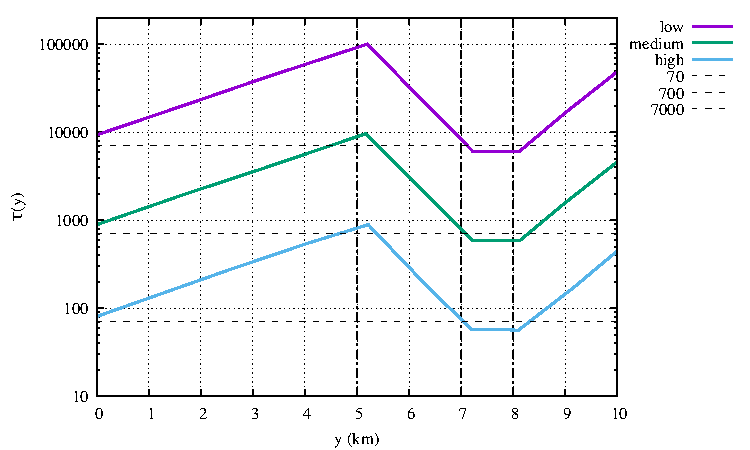
\includegraphics[width=5.25cm]{images/rheology/vvp/tau.pdf}
\includegraphics[width=5.25cm]{images/rheology/vvp/strainrates.pdf}
\includegraphics[width=5.25cm]{images/rheology/vvp/viscosities.pdf}\\
{\captionfont Obtained for $\eta_m=10^{21}$, $Y=20$MPa and $\eta_v=10^{25}$. Python code 
in images/rheology/vvp/}
\end{center}

In the following plots the resulting stress $\tau$ and effective viscosities $\eta_{eff}$
are compared between the above approach ('new') and the simpler (and naive) 
approach where $\dot\varepsilon_T$ 
is used in $\eta_{vp}$ instead of $\dot\varepsilon$ ('old'). In this particular case 
we see that it makes a difference at low strain rates close to the brittle-ductile transition.

\begin{center}
\includegraphics[width=8cm]{images/rheology/vvp/tau_comp.pdf}
\includegraphics[width=8cm]{images/rheology/vvp/viscosities_comp.pdf}\\
{\captionfont Obtained for $\eta_m=10^{21}$, $Y=20$MPa and $\eta_v=10^{25}$. Python code 
in images/rheology/vvp/}
\end{center}

\begin{remark}
The introduction of the damper $\eta_m$ in parallel with the plastic element has an unavoidable
effect: the stress $\tau$ becomes larger than $Y$ at high strain rate values! Since the $vp$ 
block is akin to a bingham fluid, this is no surprise.
\end{remark}

\begin{remark}
The viscous dashpot $\eta_v$ also acts as a maximum viscosity cutoff: if $\eta_{vp}$ becomes (very) large, i.e. $\eta_{vp} \gg \eta_v$, then $\eta_{eff} \rightarrow \eta_v$.
Conversely, if $\eta_p=Y/2\dot\varepsilon_{vp}$ becomes (very) small, i.e. $\eta_p \ll \eta_m$ then $\eta_m$ acts as a minimum viscosity limiter, i.e. $\eta_{vp} \rightarrow \eta_m$. 
Since $\eta_m \ll \eta_v$ then $\eta_{eff} \rightarrow \eta_m$.
\end{remark}

\underline{A simple regularisation} This idea originates in Massmeyer \etal (2013) \cite{madd13}. We postulate
\[
\tilde{\eta}_{eff} = \left(  1 - \exp (- \frac{\dot\varepsilon_T}{\dot\varepsilon_{T}^c}) \right)
\left( \frac{Y}{2 \dot\varepsilon_T} + \eta_m \right)
\]
where $\dot\varepsilon_{T}^c$ is the critical strain  rate at which the transition viscous to 
viscous-viscoplastic occurs given by $\dot\varepsilon_{T}^c=Y/2\eta_v$.
When $\dot\varepsilon_{T} \ll \dot\varepsilon_{T}^c$ then the exponential term tends to zero and 
\[
\tilde{\eta}_{eff} \rightarrow  \frac{Y}{2 \dot\varepsilon_T} + \eta_m 
\]
and if $\dot\varepsilon_{T} \rightarrow \infty$ then $\tilde{\eta}_{eff}\rightarrow \eta_m$.
Conversely if $\dot\varepsilon_T \rightarrow 0$ then we can carry out a Taylor expansion of the exponential 
term ($\exp x \sim 1 + x$ when $x$ is small).
\[
\tilde{\eta}_{eff} \sim \left(  \frac{\dot\varepsilon_T}{\dot\varepsilon_{T}^c} \right)
\left( \frac{Y}{2 \dot\varepsilon_T} + \eta_m \right)
\rightarrow 
\frac{\dot\varepsilon_T}{\dot\varepsilon_{T}^c}  \frac{Y}{2 \dot\varepsilon_T}  = \eta_v
\]
At low strain rates the viscosity does not 'explode' but actually converges to the background viscosity $\eta_v$.
The stress $\tau$ corresponding to this viscosity is simply $\tilde{\tau} = 2 \tilde{\eta}_{eff}$. 
Both $\tilde{\tau}$ and $ \tilde{\eta}_{eff}$ are plotted hereunder:


\begin{center}
\includegraphics[width=7.5cm]{images/rheology/vvp/tau_reg.pdf}
\includegraphics[width=7.5cm]{images/rheology/vvp/viscosities_reg.pdf}\\
{\captionfont Obtained for $\eta_m=10^{21}$, $Y=20$MPa and $\eta_v=10^{25}$. Python code 
in images/rheology/vvp/}
\end{center}


\includegraphics[width=7.5cm]{images/rheology/vvp/ratio_visc.pdf}



%which, if  yields the following effective viscosity:
%\[
%\eta_{eff} = \left( \frac{1}{\eta_M}  + \frac{1}{\frac{Y}{2 \dot{\varepsilon}_e} + \eta_m}  \right)^{-1}
%\]
%When the strain rate becomes very small,  $\dot{\varepsilon}_e \rightarrow 0$, $\eta_{eff}\rightarrow \eta_{M}$.
%When the strain rate becomes very large,  $\dot{\varepsilon}_e \rightarrow \infty$, $\eta_{eff}\rightarrow \eta_{m}$.
%We can then rewrite the above equation as a function of $\eta_{min}$ and $\eta_{max}$:
%\[
%\eta_{eff} = \left( \frac{1}{\eta_{max}}  + \frac{1}{\frac{c}{2 \dot{\varepsilon}_e} + \eta_{min}}  \right)^{-1}
%\]
%
%The effective viscosity is plotted here for various values of the minimum viscosity (for $c$=200MPa and $\eta_{max}=10^{25}Pa.s$:
%\includegraphics[width=8cm]{images/viscoplasticity/nu_eff}










